\documentclass{beamer}
%
% Choose how your presentation looks.
%
% For more themes, color themes and font themes, see:
% http://deic.uab.es/~iblanes/beamer_gallery/index_by_theme.html
%
\mode<presentation>
{
  \usetheme{default}      % or try Darmstadt, Madrid, Warsaw, ...
  \usecolortheme{default} % or try albatross, beaver, crane, ...
  \usefonttheme{default}  % or try serif, structurebold, ...
  \setbeamertemplate{navigation symbols}{}
  \setbeamertemplate{caption}[numbered]
} 
\addtobeamertemplate{navigation symbols}{}{%
	\usebeamerfont{footline}%
	\usebeamercolor[fg]{footline}%
	\hspace{1em}%
	\insertframenumber/\inserttotalframenumber
}
\setbeamertemplate{footline}{
	\hbox{%
		\begin{beamercolorbox}[wd=\paperwidth,ht=3ex,dp=1.5ex,leftskip=2ex,rightskip=2ex]{page footer}%
			\usebeamerfont{title in head/foot}%
			\insertshorttitle \hfill
			\insertsection \hfill
			\insertframenumber{} / \inserttotalframenumber
	\end{beamercolorbox}}%
}
\usepackage[english]{babel}
\usepackage[utf8x]{inputenc}
\usepackage{xcolor} % For textcolor
\usepackage{pgfplots} % For Tikz
\usepackage{media9}
\usepackage{tikz}
\usetikzlibrary{shapes,arrows}

\title[]{Flockng Algorithms for Source-Seeking Scenarios: From Double Integrators to General Non-Linear Vehicles}
\author{\textbf{Adwait Datar}}
\institute{Institute of Control Systems\\ Technical University of Hamburg\\ \vspace{1cm}This work was funded by the German Research Foundation (DFG) within their priority programme SPP 1914 Cyber-Physical Networking.}
\date{}
% \AtBeginSection[]
% {
% 	\begin{frame}
% 	\frametitle{Table of Contents}
% 	\tableofcontents[currentsection]
%	 \end{frame}
% } 

\begin{document}
\begin{frame}	
  \titlepage
\end{frame}

%Uncomment these lines for an automatically generated outline.
%\begin{frame}{Outline}
% \tableofcontents
%\end{frame}
%%%%%%%%%%%%%%%%%%%%%%%%%%%%%%%%%%%%%%%%%%%%%%%%%%%%%%%%%%%%%%%%%%%%%
\section{Flocking algorithms to address the source-seeking problem}
\subsection{Problem}
%%%%%%%%%%%%%%%%%%%%%%%%%%%%%%%%%%%%%%%%%%%%%%%%%%%%%%%%%%%%%%%%%%%%%
\begin{frame}{Source seeking problem: Abstraction}
	
\begin{itemize}
	\item A group of $N$ agents (e.g underwater robots) are deployed in the region of interest
	\item Each agent has the following properties:
	    \begin{itemize}
	        \item Absolute position measurement (e.g GPS)\footnote{This assumption can be removed as long there is relative displacement measurement}
	        \item Communication with agents within a fixed distance
	        \item Concentration measurement sensor
	        \item Computation capabilities 
	    \end{itemize}
	\item \textbf{Problem:} Design distributed control algorithms that cause the agents to flock towards the source (location with the highest concentration) in a cooperative manner.
\end{itemize}
\end{frame}
\subsection{Theory}
%%%%%%%%%%%%%%%%%%%%%%%%%%%%%%%%%%%%%%%%%%%%%%%%%%%%%%%%%%%%%%%%%%%%%
% \begin{frame}{Capabilities of a single agent (Robot)}
% \begin{itemize}
% 	\item Position information based on an indoor positioning system (can be relaxed to only distance measurements)
% 	\item Peer to peer communication and computation capabilites onboard
% 	\item Pretend to measure the strength of a virtual scalar field based on the current location
% \end{itemize}		
% \end{frame}
%%%%%%%%%%%%%%%%%%%%%%%%%%%%%%%%%%%%%%%%%%%%%%%%%%%%%%%%%%%%%%%%%%%%%
\begin{frame}{Source seeking problem as optimization}
\begin{itemize} 
	\item Look at the source seeking problem as a minimization problem
	\item Momentum methods\footnote{Polyak,1964} have been used in optimization to speed up or dampen the oscillations
	\item Naturally have momentum of the mobile robots   
	\item For theoretical analysis: Use continuous-time versions of optimization methods to study the assymptotic properties\footnote{Redont et al., 2002} 
\end{itemize}
\end{frame}
% %%%%%%%%%%%%%%%%%%%%%%%%%%%%%%%%%%%%%%%%%%%%%%%%%%%%%%%%%%%%%%%%%%%%%
% \begin{frame}{Continuous-time steepest descent with momentum}
% \begin{itemize}
% \item Consider the problem of minimizing a differentiable $f:\mathbb{R}^n\rightarrow \mathbb{R}$
% \pause
% \item The steepest descent iteration is
% \begin{equation}
% x_{k+1}=x_k - \alpha \nabla f(x_k)
% \end{equation}
% \pause
% \item The continuous-time version of the steepest descent dynamics 
% \begin{equation}
% \dot{x}= - \nabla f(x_k)
% \end{equation}
% \pause
% \item The continuous-time version of the steepest descent dynamics with momentum (also known as the heavy ball method with friction) 
% \begin{equation}
% m\ddot{x}+ \dot{x}= - \nabla f(x_k)
% \end{equation}
% \end{itemize}
% \end{frame}
%%%%%%%%%%%%%%%%%%%%%%%%%%%%%%%%%%%%%%%%%%%%%%%%%%%%%%%%%%%%%%%%%%%%%
\begin{frame}{Continuous-time Newton method with momentum}
\begin{itemize}
	\item Consider the problem of minimizing a twice-differentiable, strongly convex $f:\mathbb{R}^n\rightarrow \mathbb{R}$
	\pause
	\item The Newton iteration is
	\begin{equation}
	x_{k+1}=x_k - \alpha\nabla^2f(x_k)^{-1} \nabla f(x_k)
	\end{equation}
	\pause
	\item The continuous-time version of these dynamics can be represented as
	\begin{equation}
	\nabla^2f(x_k)\dot{x}= - \nabla f(x_k)
	\end{equation}
	\pause
	\item Adding momentum to these dynamics gives  
	\begin{equation}
	m\ddot{x}+ \nabla^2f(x_k)\dot{x}= - \nabla f(x_k)
	\end{equation}
\end{itemize}
\pause
Defining the velocity variable $v$, the dyanmics can be written as 
\begin{equation} \label{eqn: second_order_newton_cont_time}
\begin{split}
\Dot{x}&=v\\
\Dot{v}&=-k_1\nabla^2 f(x) v -k_2 \nabla f(x), 
\end{split}
\end{equation}
\end{frame}
%%%%%%%%%%%%%%%%%%%%%%%%%%%%%%%%%%%%%%%%%%%%%%%%%%%%%%%%%%%%%%%%%%%%%
\begin{frame}{Flocking and schooling in nature}

\begin{minipage}{0.45\textwidth}	
	%\hspace{0.4cm}	
	\begin{figure}
		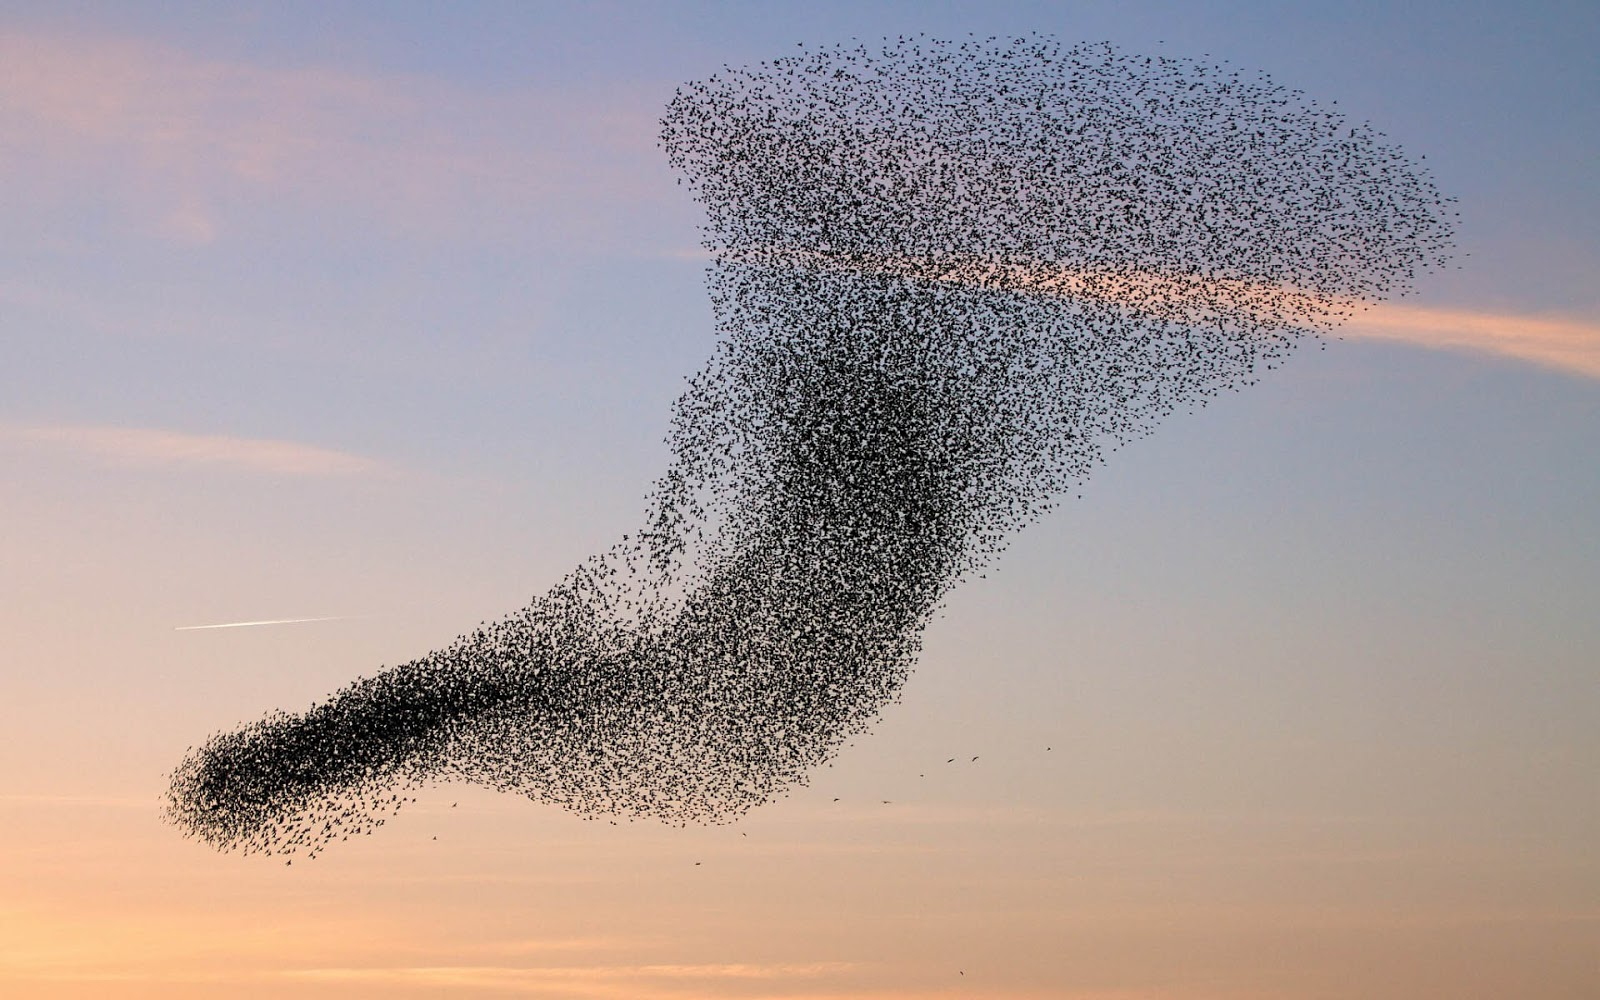
\includegraphics[width=\textwidth]{figures/flock_of_birds.jpg}
		%\caption{Fukushima Disaster}
		%\label{fig:flock_of_birds}
	\end{figure}
\end{minipage}
\hspace{0.05cm}
\begin{minipage}{0.45\textwidth}	
	\begin{figure}
		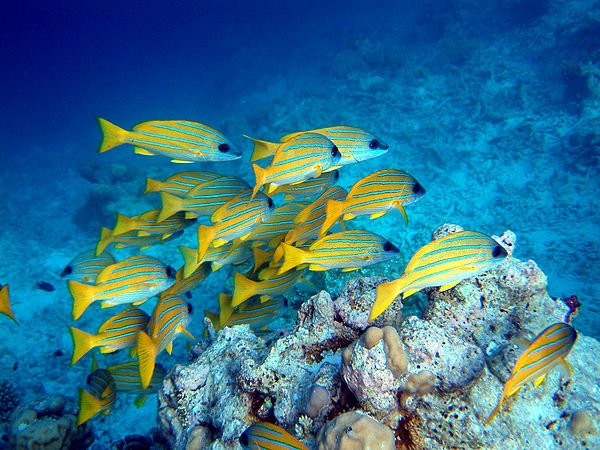
\includegraphics[width=\textwidth]{figures/schooling_fish.jpg}
		%\caption{Oil Spills}
		%\label{fig:schools_of_fish}
	\end{figure}
\end{minipage}
\begin{itemize}	
	\item The precise rules that these animals use are not known
	\item Particle-based flocking seems to be an effective approach to model such behavior
	\item In 1987, Reynold was working on animating flocking behavior where he proposed three rule
	\begin{itemize}
		\item Cohesion: Attempt to stay close to nearby neighbors
		\item Separation: Avoid collisions with nearby flockmates
		\item Alignment: attempt to match velocities with nearby flockmates
	\end{itemize}
\end{itemize}
\end{frame}
%%%%%%%%%%%%%%%%%%%%%%%%%%%%%%%%%%%%%%%%%%%%%%%%%%%%%%%%%%%%%%%%%%%%%
\begin{frame}{Flocking dynamics}
\begin{itemize}
	\item Every particle interacts with every other particle based on an interaction field $V$ which depends only on the distance between them
	\item An example of a potential field is the gravitational field $V(z)=\frac{mMG}{||z||}$
	\item Flocking dynamics\footnote{Olfati-Saber, 2004}:
	\begin{equation*}
	\begin{split}
	\Dot{q}&=p\\
	\Dot{p}&=-\nabla V(q)-\hat{L}(q)p -cp 
	\end{split}
	\end{equation*}
\end{itemize}
\end{frame}
%%%%%%%%%%%%%%%%%%%%%%%%%%%%%%%%%%%%%%%%%%%%%%%%%%%%%%%%%%%%%%%%%%%%%
\begin{frame}{Flocking towards the source}
\begin{itemize}
\item Consider now an underlying source field $\psi:\mathbf{R}^m \xrightarrow{} \mathbf{R}$ which is smooth enough and convex.
\item Add a forcing term to the flocking dynamics motivated from the discussion on optimization
\item Flocking dynamics with source-seeking:
\begin{equation*}
\begin{split}
\Dot{q}&=p\\
\Dot{p}&=-\nabla V(q)-\hat{L}(q)p -cp\textcolor{red}{-k_1\nabla^2 \Psi(q) p -k_2 \nabla \Psi(q)}
\end{split}
\end{equation*}
\end{itemize}
\end{frame}
%%%%%%%%%%%%%%%%%%%%%%%%%%%%%%%%%%%%%%%%%%%%%%%%%%%%%%%%%%%%%%%%%%%%%
\begin{frame}{Stability(Convergence) Analysis}
	Flocking dynamics with source-seeking:
	\begin{equation*}
	\begin{split}
	\Dot{q}&=p\\
	\Dot{p}&=-\nabla V(q)-\hat{L}(q)p -cp\textcolor{red}{-k_1\nabla^2 \Psi(q) p -k_2 \nabla \Psi(q)}
	\end{split}
	\end{equation*}
\textbf{Theorem 1} For twice differentiable convex fields $\psi:\mathbf{R}^m \xrightarrow{} \mathbf{R}$, the above flocking dynamics are stable i.e the trajectories remain bounded. Moreover, for all initial conditions $(q(0),p(0))$, the trajectories converge asymptotically to the set $$\mathcal{W}:=\{(q^*,0)|\nabla V (q^*)+ k_2\nabla\Psi(q^*) = 0 \}.$$
%% Additionally, if $\psi$ is radially symmetric about the source $q_s$, then, at the equilibrium of the translational dynamics of the center of mass, (?), $q_s \in \textnormal{convhull}(q^*)$  
\textbf{Corollary 1} Assume, the field $\psi:\mathbf{R}^m \xrightarrow{} \mathbf{R}$ is strictly convex, quadratic and has a unique minimum located at $q_s$, we have that $\lim_{t\rightarrow \infty}q_c(t)=q_s$.

\end{frame}
%%%%%%%%%%%%%%%%%%%%%%%%%%%%%%%%%%%%%%%%%%%%%%%%%%%%%%%%%%%%%%%%%%%%%%
%\begin{frame}{Stability(Convergence) Analysis}
%\textbf{Proof:}
%	\begin{itemize}
%		\item Define the energy function
%		\begin{equation*}\label{eqn: energy function}
%		E(t):= V(q(t)) + k_2\Psi(q(t)) + \frac{1}{2}p(t)^Tp(t).
%		\end{equation*}
%		%\pause
%		\item Differentiating w.r.t time, 
%		\begin{equation*}
%		\begin{split}
%		\dot{E}&= (\nabla V(q) + k_2\nabla \Psi(q))^T\dot{q} + p^T\dot{p} \\
%		&=-p^T(\hat{L}(q)+cI+k_1\nabla^2\Psi(q))p\\
%		&\leq 0.
%		\end{split}
%		\end{equation*}
%		%\pause
%		\item $E(t)\leq E(0) ~\forall t\geq0$ implies the boundedness of trajectories
%		%\pause
%		\item  $\dot{E}=0 \iff p=0$. Thus, LaSalle's invariance principle $\implies$ that the trajectories converge to the largest invariant set contained in $\mathcal{W}:=\{(q^*,0)|\nabla V (q^*)+ k_2\nabla \Psi(q^*) = 0 \}$
%		%\pause
%		%\item At equilibrium of the center of mass dynamics, $q^*$ satisfies $\frac{k_2}{N}(\mathbf{1}_N\otimes I_m)^T\nabla\Psi(q)$
%	\end{itemize}
%\end{frame}
%%%%%%%%%%%%%%%%%%%%%%%%%%%%%%%%%%%%%%%%%%%%%%%%%%%%%%%%%%%%%%%%%%%%%
% \begin{frame}{Stability(Convergence) Analysis}
% 	\textbf{Sketch of the proof(ctd):}
% 	\begin{itemize}
% 		\item To characterize the equilibrium, we write the dynamics of the center of mass
% 		\begin{equation} \label{eqn: COM flocking dynamics}
% 		\begin{split}
% 		\Dot{q}_c&=p_c\\
% 		\Dot{p}_c&=-cp_c-\frac{1}{N}(\mathbf{1}_N\otimes I_m)^T(k_1\nabla^2\Psi(q) p +k_2 \nabla\Psi(q)) 
% 		\end{split}
% 		\end{equation}
% 		\pause
% 		\item $\lim_{t\rightarrow \infty}p(t)=0 \implies \lim_{t\rightarrow \infty}p_c(t)=0$
		
% 	\end{itemize}
% \end{frame}
%%%%%%%%%%%%%%%%%%%%%%%%%%%%%%%%%%%%%%%%%%%%%%%%%%%%%%%%%%%%%%%%%%%%%
%\begin{frame}{Stability(Convergence) Analysis}
%\textbf{Corollary 1} Assume, the field $\psi:\mathbf{R}^m \xrightarrow{} \mathbf{R}$ is strictly convex, quadratic and has a unique minimum located at $q_s$, we have that $\lim_{t\rightarrow \infty}q_c(t)=q_s$.
%
%%\pause
%\textbf{Proof:}
%	\begin{itemize}
%	    \item For quadratic $\psi(q)=\frac{1}{2}q^THq+g^Tq+c_0$, with $H\succ 0$, the source is the unique solution to $Hq_s+g=0$
%		%\pause
%	    \item The center of mass dynamics are governed by
%		    \begin{equation} \label{eqn: COM flocking dynamics}
%        		\begin{split}
%        		\Dot{q}_c&=p_c\\
%        		\Dot{p}_c&=-cp_c-\frac{1}{N}(\mathbf{1}_N\otimes I_m)^T(k_1\nabla^2\Psi(q) p +k_2 \nabla\Psi(q)) 
%        		\end{split}
%		    \end{equation}
%	    %\pause
%	    \item $\frac{1}{N}(\mathbf{1}_N\otimes I_m)^T\nabla\Psi(q)=0$
%		%\pause
%		\item At equilibrium $q^*$, 
%		\begin{equation*}
%		\begin{split}
%		\frac{1}{N}\sum_{i=1}^{N}\nabla\psi(q_i^*)&=0 \iff \textnormal{i.e } H(\frac{1}{N}\sum_{i=1}^{N}q_i^*)+g=0\\
%		\textnormal{i. e  } Hq_c^*+g&=0 \iff q_c^*=q_s
%		\end{split}	
%		\end{equation*}
%		\end{itemize}
%\end{frame}
%\subsection{Practical aspects}
%%%%%%%%%%%%%%%%%%%%%%%%%%%%%%%%%%%%%%%%%%%%%%%%%%%%%%%%%%%%%%%%%%%%%%
%\begin{frame}{Remarks on Plausibility of Assumptions}
%Assumption for theoretical analysis:
%\begin{itemize}
%	\item A1: Agents are modeled as double integrators
%	\item A2: The scalar field is assumed to be convex and twice differentiable
%	\item A3: Measurements of $\psi(q_i)$, $\nabla \psi(q_i)$ and $\nabla^2\psi(q_i)$ by agent $i$
%\end{itemize}
%\end{frame}
%%%%%%%%%%%%%%%%%%%%%%%%%%%%%%%%%%%%%%%%%%%%%%%%%%%%%%%%%%%%%%%%%%%%%
\begin{frame}{Towards Experiments: Modeling agents as double integrators}
\begin{figure}[h!]
	\tikzstyle{block} = [draw, rectangle, 
    minimum height=3em, minimum width=6em]
\tikzstyle{sum} = [draw,  circle, node distance=1cm]
\tikzstyle{input} = [coordinate]
\tikzstyle{output} = [coordinate]
\tikzstyle{pinstyle} = [pin edge={to-,thin,black}]

% The block diagram code is probably more verbose than necessary
%\begin{tikzpicture}[auto, node distance=2cm,>=latex']
%    % We start by placing the blocks
%    \node [input, name=input] {};
%    \node [sum, right of=input] (sum) {};
%    \node [block, right of=sum] (controller) {Controller};
%    \node [block, right of=controller, pin={[pinstyle]above:Disturbances},
%            node distance=3cm] (system) {System};
%    % We draw an edge between the controller and system block to 
%    % calculate the coordinate u. We need it to place the measurement block. 
%    \draw [->] (controller) -- node[name=u] {$u$} (system);
%    \node [output, right of=system] (output) {};
%    \node [block, below of=u] (measurements) {Measurements};
%
%    % Once the nodes are placed, connecting them is easy. 
%    \draw [draw,->] (input) -- node {$r$} (sum);
%    \draw [->] (sum) -- node {$e$} (controller);
%    \draw [->] (system) -- node [name=y] {$y$}(output);
%    \draw [->] (y) |- (measurements);
%    \draw [->] (measurements) -| node[pos=0.99] {$-$} 
%        node [near end] {$y_m$} (sum);
%\end{tikzpicture}

\begin{tikzpicture}[auto, node distance=2cm,>=latex']
% We start by placing the blocks
\node [input, name=input] {};
\node [block, right of=input,pin={[pinstyle]above:$\Psi(q)$},node distance=2.5cm](Flockcontrol) {$u=-\nabla V-(\hat{L}+cI)p + f_{\gamma} $};
\node [block, right of=Flockcontrol,node distance=3cm,minimum height=1em,minimum width=2em](integrator) {$\frac{1}{s}$};
\node [block, right of=integrator,node distance=2cm,minimum height=2.5em,minimum width=3em](velocityloop) {$G_{\textnormal{vel}}$};
\node [output, right of=velocityloop,node distance=1cm](output) {};
\node [block, below of=integrator,node distance=2cm](network) {Network};
% Once the nodes are placed, connecting them is easy. 
\draw [draw,->] (input) -- node {} (Flockcontrol);
\draw [draw,->] (Flockcontrol) -- node {} (integrator);
\draw [draw,->] (integrator) -- node {$p_{\textnormal{des}}$} (velocityloop);
\draw [draw,->] (velocityloop) -- node[name=outmid] {$\begin{bmatrix}q\\p\end{bmatrix}$} (output);
\draw [->] (outmid) |- (network);
\draw [-] (network) -| (input);
\end{tikzpicture}
	\caption{Control Architecture}
	\label{fig:control_arch}	
\end{figure}
\begin{itemize}
	\item The flocking loop is runs at 20Hz 
	\item $G_{\textnormal{vel}}$: closed loop velocity tracking loop runs at 100Hz
	\item Initial tests show that the velocity controller is fast enough $\implies$ approximate $G_{\textnormal{vel}}$ by single integrator dynamics.
\end{itemize}
\end{frame}
%%%%%%%%%%%%%%%%%%%%%%%%%%%%%%%%%%%%%%%%%%%%%%%%%%%%%%%%%%%%%%%%%%%%%%
%\begin{frame}{Towards Experiments: Convexity and differentiability of field}
%
%\begin{itemize}
%    \item The actual fields in the scenarios of interest will most likely not be convex and perhaps not smooth enough
%    \item Non-differentiability: Fit a locally smooth approximation
%    \item Non-convexity: The result can then be seen as a local convergence result
%    \item Experimental tests include log-convex fields and fields with 2 minima to probe the applicability of the algorithm when the assumption is violated.
%\end{itemize}
%\end{frame}
%%%%%%%%%%%%%%%%%%%%%%%%%%%%%%%%%%%%%%%%%%%%%%%%%%%%%%%%%%%%%%%%%%%%%
\begin{frame}{Towards Experiments: $\psi(q_i)$, $\nabla \psi(q_i)$, $\nabla^2\psi(q_i)$}
\begin{figure}[h!]	
		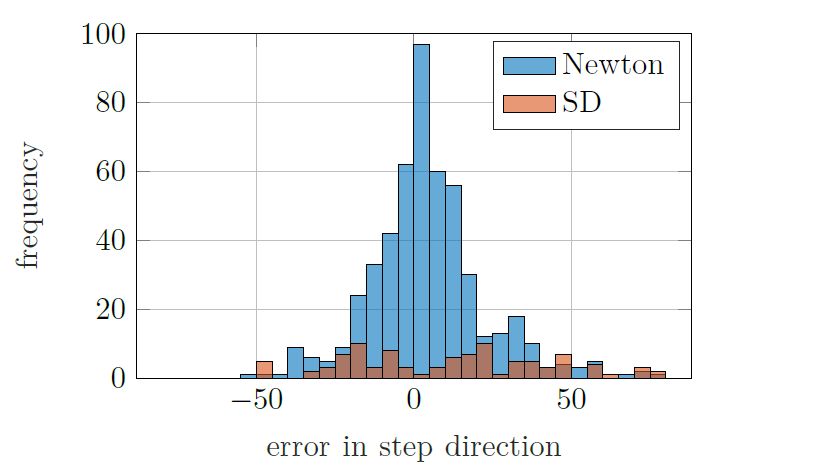
\includegraphics[width=7cm]{figures/newton_SD_direction.png}
		%\caption{Histograms of errors (in angles) between the estimated and true gradient direction and modified Newton step direction when the field measurements are corrupted}
		\label{fig:direction_errors_noise}
	\end{figure}
\begin{itemize}
	\item Corrupt the field strength measurement by +/- 5 percent of the field strength. 
	\item Estimate gradient by collecting local data and solving a least squares problem
	\item Estimate the hessian by collecting data from neighbors and solving another least squares problem
	\item Heuristic: Use Steepest Descent until the estimated hessian is positive definite.
\end{itemize}
\end{frame}
%%%%%%%%%%%%%%%%%%%%%%%%%%%%%%%%%%%%%%%%%%%%%%%%%%%%%%%%%%%%%%%%%%%%%
\subsection{Experimental Results}
%%%%%%%%%%%%%%%%%%%%%%%%%%%%%%%%%%%%%%%%%%%%%%%%%%%%%%%%%%%%%%%%%%%%%
\begin{frame}{Indoor experimental setup}

\begin{minipage}{0.55\textwidth}	
    \begin{figure}[h!]
	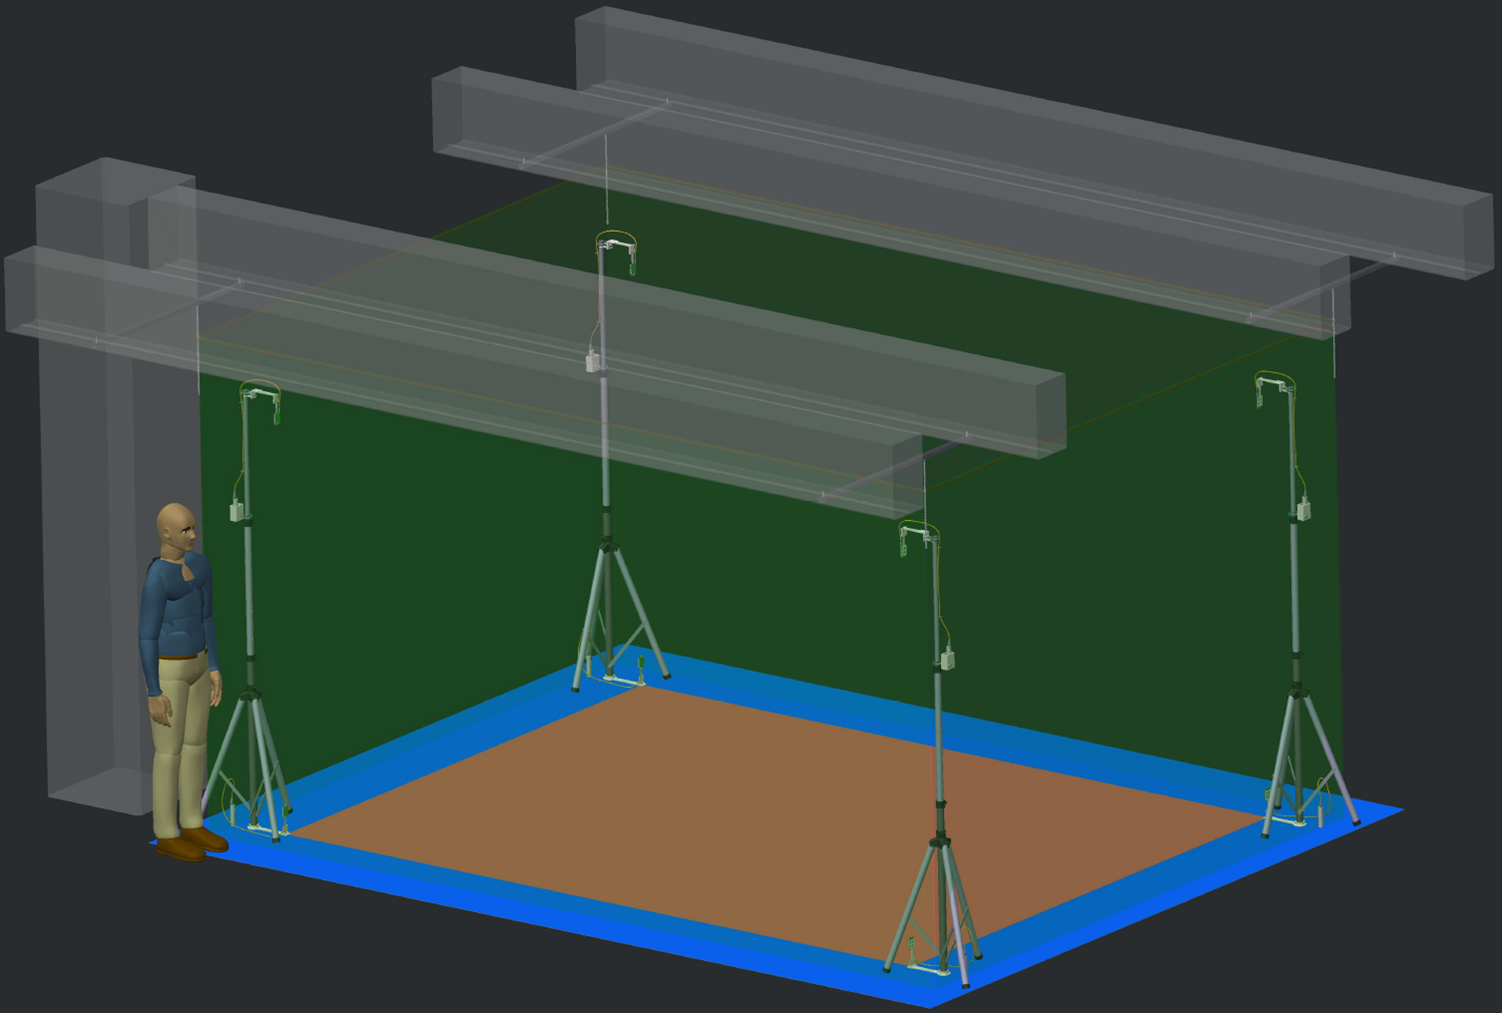
\includegraphics[width=6cm]{figures/LPS_Setup.png}
	\caption{LPS Setup}
	\label{fig:control_arch}	
\end{figure}		
\end{minipage}
	\hspace{0.05cm}
\begin{minipage}{0.35\textwidth}
    \begin{figure}[h!]
	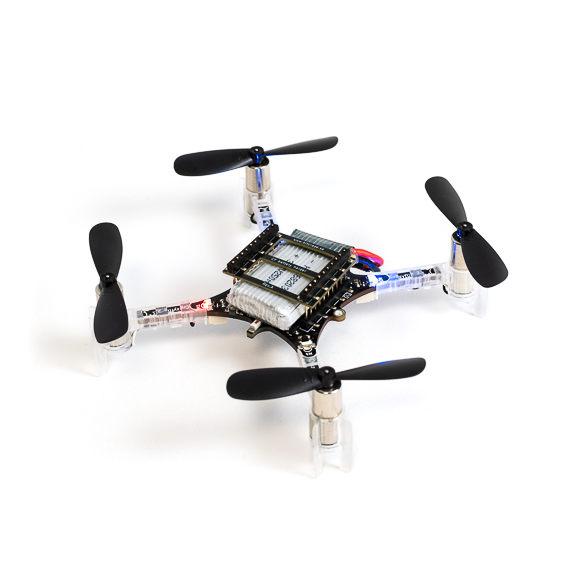
\includegraphics[width=4cm]{figures/crazyflie_2_1_585px.jpg}
	\caption{Crazyflie 2.1}
	\label{fig:control_arch}	
\end{figure}		
\end{minipage}

\begin{itemize}
	\item Indoor Positioning System called the Loco Position System (LPS) and Crazyflie 2.0 developed by the company bitcraze\footnote{https://www.bitcraze.io/products/crazyflie-2-1/}
	\item Implemented a peer-to-peer communication protocol \footnote{Paulsen, 2018.Master thesis.}
\end{itemize}
\end{frame}
%%%%%%%%%%%%%%%%%%%%%%%%%%%%%%%%%%%%%%%%%%%%%%%%%%%%%%%%%%%%%%%%%%%%%%
%\begin{frame}{Experimental results: Quadratic field}
%$\psi(q)=(q-c)^T\begin{bmatrix}1&0\\0&2\end{bmatrix}(q-c)$ with $c=\begin{bmatrix}2\\1.5\end{bmatrix}$
%\vspace{5cm}
%\end{frame}
%%%%%%%%%%%%%%%%%%%%%%%%%%%%%%%%%%%%%%%%%%%%%%%%%%%%%%%%%%%%%%%%%%%%%%
%\begin{frame}{Experimental results: Log-convex field}
%$\psi(q)=-\textnormal{exp}(-||q-c||^2)$ with $c=\begin{bmatrix}2\\1.5\end{bmatrix}$
%\vspace{5cm}	
%\end{frame}
%%%%%%%%%%%%%%%%%%%%%%%%%%%%%%%%%%%%%%%%%%%%%%%%%%%%%%%%%%%%%%%%%%%%%%
%\begin{frame}{Experimental results: Field with two minima}
%$\psi(q)=-\textnormal{exp}(-||q-c_1||^2)-\textnormal{exp}(-||q-c_2||^2)$ with $c_1=\begin{bmatrix}1\\1\end{bmatrix}$, $c_2=\begin{bmatrix}3\\2\end{bmatrix}$
%\vspace{5cm}	
%\end{frame}
%%%%%%%%%%%%%%%%%%%%%%%%%%%%%%%%%%%%%%%%%%%%%%%%%%%%%%%%%%%%%%%%%%%%%%
%\begin{frame}{Visualizing experimental results}
%
%\end{frame}
%%%%%%%%%%%%%%%%%%%%%%%%%%%%%%%%%%%%%%%%%%%%%%%%%%%%%%%%%%%%%%%%%%%%%
% \begin{frame}{Experimental results: Quadratic field}
% 	\textcolor{red}{Replace figure with animation and video} 
% 	\begin{figure}[h!]	
% 		\includegraphics[width=12cm]{figures/quadratic_field_contour.png}
% 		%\caption{Histograms of errors (in angles) between the estimated and true gradient direction and modified Newton step direction when the field measurements are corrupted}
% 		\label{fig:quadratic_field}
% 	\end{figure}
% \end{frame}
%%%%%%%%%%%%%%%%%%%%%%%%%%%%%%%%%%%%%%%%%%%%%%%%%%%%%%%%%%%%%%%%%%%%%
% \begin{frame}{Experimental results: Log-convex field}
% 	\textcolor{red}{Replace figure with animation and video}
% 	\begin{figure}[h!]	
% 		\includegraphics[width=12cm]{figures/log_convex_field_contour.png}
% 		%\caption{Histograms of errors (in angles) between the estimated and true gradient direction and modified Newton step direction when the field measurements are corrupted}
% 		\label{fig:log_convex_field}
% 	\end{figure}
% \end{frame}
%%%%%%%%%%%%%%%%%%%%%%%%%%%%%%%%%%%%%%%%%%%%%%%%%%%%%%%%%%%%%%%%%%%%%
% \begin{frame}{Experimental results: Non-convex field}
% 	\textcolor{red}{Replace figure with animation and video}
% 	\begin{figure}[h!]	
% 		\includegraphics[width=12cm]{figures/non_convex_field_contour.png}
% 		%\caption{Histograms of errors (in angles) between the estimated and true gradient direction and modified Newton step direction when the field measurements are corrupted}
% 		\label{fig:non_convex_field}
% 	\end{figure}
% \end{frame}
%%%%%%%%%%%%%%%%%%%%%%%%%%%%%%%%%%%%%%%%%%%%%%%%%%%%%%%%%%%%%%%%%%%%%%
% \begin{frame}{Experimental Results: Quadratic field(Video)}
% \includemedia[
% activate=pageopen,
% width=300pt,height=200pt,
% addresource=animations/OBLIQUE_quadratic_mod_newton_Fig_4.mp4,
% flashvars={%
% 	src=figures/noObstacle.mp4      % same path as in addresource!
% 	%&scaleMode=stretch % removes black bars
% 	&autoPlay=true      % optional configuration
% 	&loop=true          % variables
% }
% ]{}{StrobeMediaPlayback.swf}
% \end{frame}
% %%%%%%%%%%%%%%%%%%%%%%%%%%%%%%%%%%%%%%%%%%%%%%%%%%%%%%%%%%%%%%%%%%%%%%
% \begin{frame}{Experimental Results: Quadratic field(Animation)}

% 		\includemedia[
% 		activate=pageopen,
% 		width=300pt,height=200pt,
% 		addresource=animations/convex.mp4,
% 		flashvars={%
% 			src=figures/noObstacle.mp4      % same path as in addresource!
% 			%&scaleMode=stretch % removes black bars
% 			&autoPlay=true      % optional configuration
% 			&loop=true          % variables
% 		}
% 		]{}{StrobeMediaPlayback.swf}

% \end{frame}
% %%%%%%%%%%%%%%%%%%%%%%%%%%%%%%%%%%%%%%%%%%%%%%%%%%%%%%%%%%%%%%%%%%%%%%
% \begin{frame}{Experimental Results: Log-Convex quadratic field (Video)}
% 		\includemedia[
% 		activate=pagevisible,
% 		width=300pt,height=200pt,
% 		addresource=animations/OBLIQUEVIEW__log_convex_mod_newton_Fig_5.mp4,
% 		flashvars={%
% 			src=figures/noObstacle.mp4      % same path as in addresource!
% 			%&scaleMode=stretch % removes black bars
% 			&autoPlay=true      % optional configuration
% 			&loop=true          % variables
% 		}
% 		]{}{StrobeMediaPlayback.swf}
% \end{frame}
% %%%%%%%%%%%%%%%%%%%%%%%%%%%%%%%%%%%%%%%%%%%%%%%%%%%%%%%%%%%%%%%%%%%%%%
% \begin{frame}{Experimental Results: Log-Convex quadratic field (Animation)}
% 	\includemedia[
% 	activate=pagevisible,
% 	width=300pt,height=200pt,
% 	addresource=animations/quasiConvex.mp4,
% 	flashvars={%
% 		src=figures/noObstacle.mp4      % same path as in addresource!
% 		%&scaleMode=stretch % removes black bars
% 		&autoPlay=true      % optional configuration
% 		&loop=true          % variables
% 	}
% 	]{}{StrobeMediaPlayback.swf}
% \end{frame}
% %%%%%%%%%%%%%%%%%%%%%%%%%%%%%%%%%%%%%%%%%%%%%%%%%%%%%%%%%%%%%%%%%%%%%%
% \begin{frame}{Experimental Results: Field with multiple minima (Video)}
% 	\includemedia[
% 	activate=pageopen,
% 	width=300pt,height=200pt,
% 	addresource=animations/2 minima mod Newton noise.mp4,
% 	flashvars={%
% 		src=figures/noObstacle.mp4      % same path as in addresource!
% 		%&scaleMode=stretch % removes black bars
% 		&autoPlay=true      % optional configuration
% 		&loop=true          % variables
% 	}
% 	]{}{StrobeMediaPlayback.swf}
% \end{frame}
% %%%%%%%%%%%%%%%%%%%%%%%%%%%%%%%%%%%%%%%%%%%%%%%%%%%%%%%%%%%%%%%%%%%%%%
% \begin{frame}{Experimental Results: Field with multiple minima (Animation)}
% 	\includemedia[
% 	activate=pageopen,
% 	width=300pt,height=200pt,
% 	addresource=animations/2minima.mp4,
% 	flashvars={%
% 		src=figures/noObstacle.mp4      % same path as in addresource!
% 		%&scaleMode=stretch % removes black bars
% 		&autoPlay=true      % optional configuration
% 		&loop=true          % variables
% 	}
% 	]{}{StrobeMediaPlayback.swf}
% \end{frame}
%%%%%%%%%%%%%%%%%%%%%%%%%%%%%%%%%%%%%%%%%%%%%%%%%%%%%%%%%%%%%%%%%%%%%
%%\subsection{Conclusion}
%%%%%%%%%%%%%%%%%%%%%%%%%%%%%%%%%%%%%%%%%%%%%%%%%%%%%%%%%%%%%%%%%%%%%
\begin{frame}{Conclusions and ongoing work}
Conclusions:
\begin{itemize}
    \item Proposed a distributed control algorithm to address the source-seeking probem
    \item Analyzed the convergence properties
    \item Presented experimental results
\end{itemize}
Ongoing Work:
\begin{itemize}
    \item Consider general non-linear agent dynamics instead of approximating it as a single integrator\footnote{A.  Attallah,  A.  Datar,  and  H.  Werner,  “Flocking  of  linear  parametervarying agents: Source seeking application with underwater vehicles (To be presented at IFAC 2020).}
    \item Consider level-tracking scenarios
    % \footnote{\textcolor{red}{Preliminary results: youtube link}}
\end{itemize}
\end{frame}
%%%%%%%%%%%%%%%%%%%%%%%%%%%%%%%%%%%%%%%%%%%%%%%%%%%%%%%%%%%%%%%%%%%%%
\subsection{(Speculative) Extension to non-linear/uncertain agents} 
%%%%%%%%%%%%%%%%%%%%%%%%%%%%%%%%%%%%%%%%%%%%%%%%%%%%%%%%%%%%%%%%%%%%%
%%%%%%%%%%%%%%%%%%%%%%%%%%%%%%%%%%%%%%%%%%%%%%%%%%%%%%%%%%%%%%%%%%%%%
\subsubsection{Double integrator agents to general non-linear agents}
\begin{frame}{Double integrator agents to general non-linear agents}
	\begin{figure}[h!]
		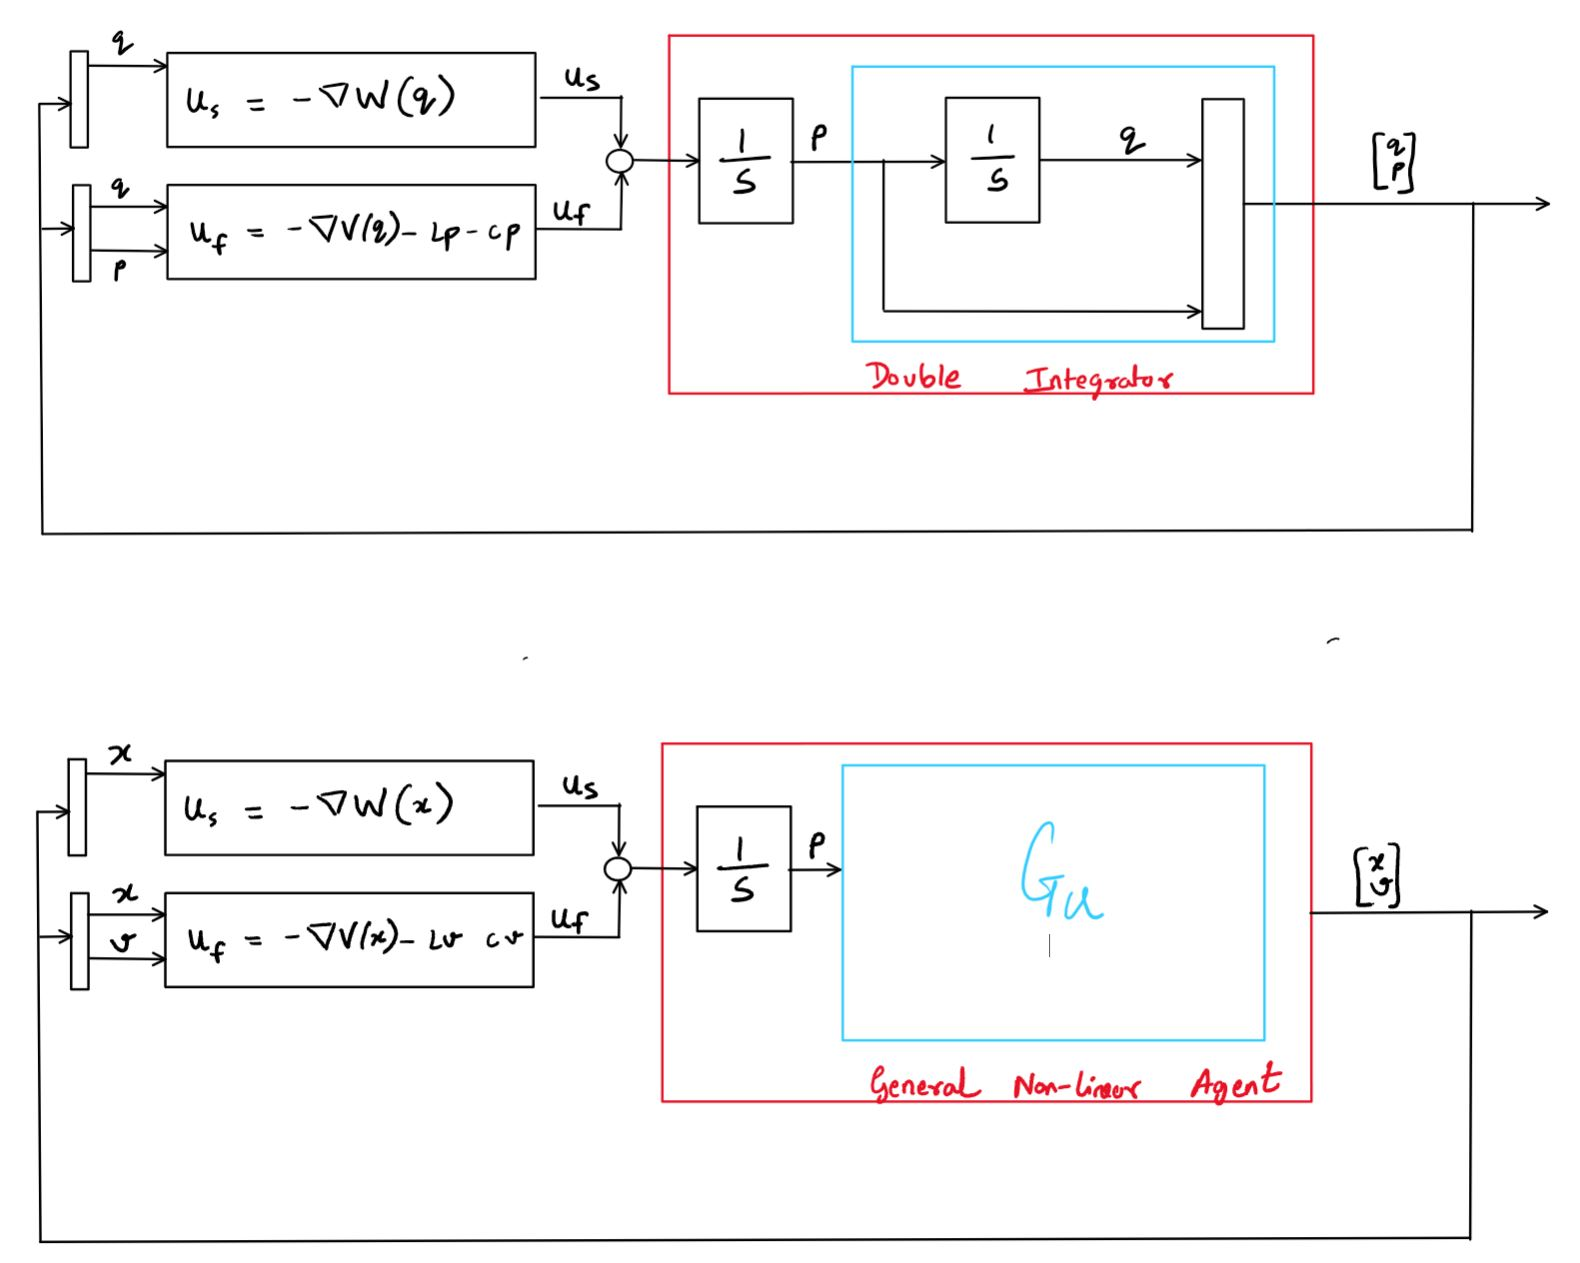
\includegraphics[width=10cm]{doc/1_Flocking_source_seek/double_integrator_to_general_agents_slide.jpg}
		%\caption{}
		\label{fig:control_arch}	
	\end{figure}	
\end{frame}
%%%%%%%%%%%%%%%%%%%%%%%%%%%%%%%%%%%%%%%%%%%%%%%%%%%%%%%%%%%%%%%%%%%%%
\begin{frame}{Double integrator agents to general non-linear agents}
Dynamics with double integrator:
\begin{equation*}
\begin{split}
\Dot{q}&=p\\
\Dot{p}&=-\nabla V(q)-\hat{L}(q)p -cp\textcolor{red}{-k_1\nabla^2 \Psi(q) p -k_2 \nabla \Psi(q)}
\end{split}
\end{equation*}	
Dynamics with general agents:
\begin{equation*}
\begin{split}
\begin{bmatrix}
x\\v
\end{bmatrix}&=G_{\textnormal{cl}}p\\
\Dot{q}&=p\\
\Dot{p}&=-\nabla V(\textcolor{blue}{x})-\hat{L}(\textcolor{blue}{x})\textcolor{blue}{v} -c\textcolor{blue}{v}\textcolor{red}{-k_1\nabla^2 \Psi(\textcolor{blue}{x}) \textcolor{blue}{v} -k_2 \nabla \Psi(\textcolor{blue}{x})}
\end{split}
\end{equation*}			
\end{frame}
%%%%%%%%%%%%%%%%%%%%%%%%%%%%%%%%%%%%%%%%%%%%%%%%%%%%%%%%%%%%%%%%%%%%%
\begin{frame}{Double integrator agents to general non-linear agents}
\textbf{Core Idea:}
\\
Under  
\begin{itemize}
\item a Lipschitz condition on the underlying scalar field 
\item a Lipschitz condition on the interaction field
\item $L_2$ bound on the tracking error of the local closed loop, $G_{\textnormal{cl}}$
\end{itemize}
the dynamics for general agents could be written as:
\begin{equation*}
\begin{split}
\Dot{q}&=p\\
\Dot{p}&=-\nabla V(q)-\hat{L}(q)p -cp\textcolor{red}{-k_1\nabla^2 \Psi(q) p -k_2 \nabla \Psi(q)} + \textcolor{blue}{d}\\
||d_T||&\leq K ||p_T||_{L_2} \forall T
\end{split}
\end{equation*}	
\begin{itemize}
\item Standard dissipativity based arguments to show stability (Boundedness of trajectories)
\item Assymptotic stability not shown !
\end{itemize}
\end{frame}
%%%%%%%%%%%%%%%%%%%%%%%%%%%%%%%%%%%%%%%%%%%%%%%%%%%%%%%%%%%%%%%%%%%%%
\begin{frame}{Double integrator agents to general non-linear agents}
A speculative idea
\begin{itemize}
	\item IQCs can be used efficiently to get upper bounds on robust exponential decay rates\footnote{Boczar, R., Lessard, L., Packard, A. and Recht, B., 2017. Exponential stability analysis via integral quadratic constraints. arXiv preprint arXiv:1706.01337.}
	\item Can be possibly applied to LPV systems to obtain exponential decay rates under parameter variation
	\item These rates could be then used with a singular perturbation and a regular perturbation argument to prove asymptotic stability of the overall system
	\item The linear analogue would be to consider the slowest eigen values of the closed loop agent dynamics
\end{itemize}
\end{frame}
%%%%%%%%%%%%%%%%%%%%%%%%%%%%%%%%%%%%%%%%%%%%%%%%%%%%%%%%%%%%%%%%%%%%%
\begin{frame}{Other speculative ideas}
	\
	\begin{itemize}
		\item Adapt the flocking algorithm coefficients online based on the measured error such the $\dot{E}<0$. (Borrowing ideas from adaptive control)
		\item Similar to ideas in \footnote{Chopra, N. and Spong, M.W., 2006. Passivity-based control of multi-agent systems. In Advances in robot control (pp. 107-134). Springer, Berlin, Heidelberg.}, design local tracking control for passivity and use the fact the interconnections of passive systems is passive.
	\end{itemize}
\end{frame}
%%%%%%%%%%%%%%%%%%%%%%%%%%%%%%%%%%%%%%%%%%%%%%%%%%%%%%%%%%%%%%%%%%%%%
%%%%%%%%%%%%%%%%%%%%%%%%%%%%%%%%%%%%%%%%%%%%%%%%%%%%%%%%%%%%%%%%%%%%%
%\begin{frame}{Other directions we have in mind}
%	\begin{itemize}
%		\item Scalable Analysis of consensus via IQCs \footnote{Khong, S.Z., Lovisari, E. and Rantzer, A., 2016. A unifying framework for robust synchronization of heterogeneous networks via integral quadratic constraints. IEEE Transactions on Automatic Control, 61(5), pp.1297-1309.}
%		\item Stochastic version of IQCs for analyzing lossy consensus \footnote{Hu, B., Seiler, P. and Rantzer, A., 2017. A unified analysis of stochastic optimization methods using jump system theory and quadratic constraints. arXiv preprint arXiv:1706.08141.}
%	\end{itemize}
%\end{frame}
%%%%%%%%%%%%%%%%%%%%%%%%%%%%%%%%%%%%%%%%%%%%%%%%%%%%%%%%%%%%%%%%%%%%%
\begin{frame}{}
\begin{center}
    \huge{Thank you}
\end{center}
\end{frame}
%%%%%%%%%%%%%%%%%%%%%%%%%%%%%%%%%%%%%%%%%%%%%%%%%%%%%%%%%%%%%%%%%%%%%
%%%%%%%%%%%%%%%%%%%%%%%%%%%%%%%%%%%%%%%%%%%%%%%%%%%%%%%%%%%%%%%%%%%%%

\end{document}
